\chapter{Equipamiento usado para correr las pruebas}
\label{testbench}

Para realizar las pruebas de performance se utilizaron diversos nodos de computo, de diversos lugares que
gentilmente proveyeron tiempo de CPU para poder correr estos trabajos

Las pruebas de GPU se realizaron en las siguientes maquinas.
\begin{itemize}
  \item CECAR - GPU2: 2 x AMD Opteron 6320 - 64GB DDR3 - NVIDIA Tesla K40
  \item CECAR - GPU0: 2 x AMD Opteron 6320 - 64GB DDR3 - 2 x NVIDIA Tesla M2090
  \item GIOL - GNODE01: 8 x AMD Opteron 6276 - 128GB DDR3 - 4 x NVIDIA Tesla M2090
  \item FFYB - LAB8: Intel Core i5-3330 @ 3.0 Ghz - 8GB DDR3 - 2 x GeForce GTX 780
  \item FFYB - LAB7: Intel Core i5-3330 @ 3.0 Ghz - 8GB DDR3 - GeForce GTX 580 - GeForce GTX 780
\end{itemize}

Estas maquinas contaron con el siguiente software:
\begin{itemize}
  \item Intel C/C++ Compiler 2013
  \item Intel Fortran Compiler 2013
  \item Intel MKL 2013
  \item Nvidia CUDA 6.0
\end{itemize}

Las opciones de compilaci\'on usadas para CUDA fueron:
\textit{}

Las pruebas de CPU se realizaron en las siguientes maquinas:
\begin{itemize}
  \item SIASA - Host: 2 x Intel Xeon E5-2620 v2 - 32GB DDR3 - Intel Xeon Phi
\end{itemize}

Estas maquinas contaron con el siguiente software:
\begin{itemize}
  \item Intel C/C++ Compiler 2015
  \item Intel Fortran Compiler 2015
  \item Intel MKL 2015
\end{itemize}

\chapter{Descripci\'on de modelos qu\'imicos probados}
\label{detalle-grupos}

\section*{Hemoglobina}
\begin{figure}[htbp]
   \centering
   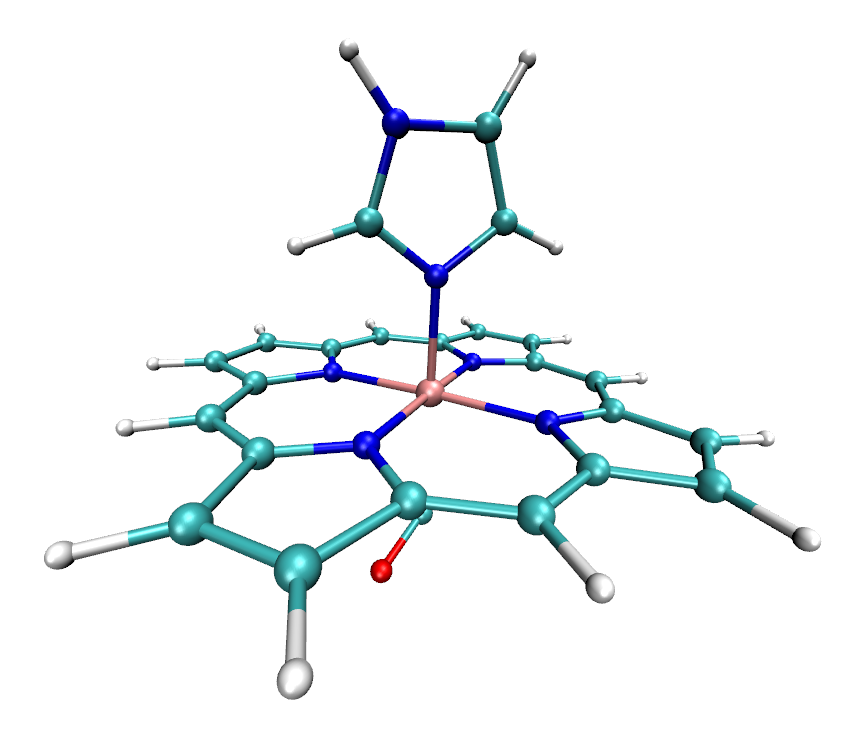
\includegraphics[width=\plotwidth]{images/hemo.png}
   \caption{Render de Hemo}
   \label{fig:render-hemo}
\end{figure}


\section*{Fullerno $C_{60}$}
\begin{figure}[htbp]
   \centering
   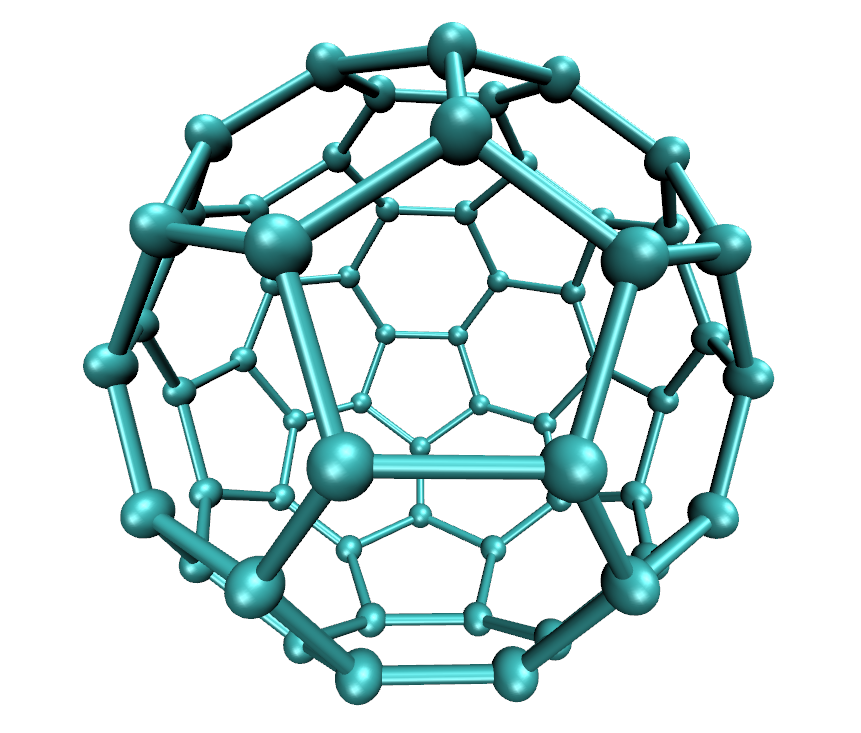
\includegraphics[width=\plotwidth]{images/fullereno.png}
   \caption{Render de fullereno $C_{60}$}
   \label{fig:render-fullereno}
\end{figure}


\section*{Caroteno}
\begin{figure}[htbp]
   \centering
   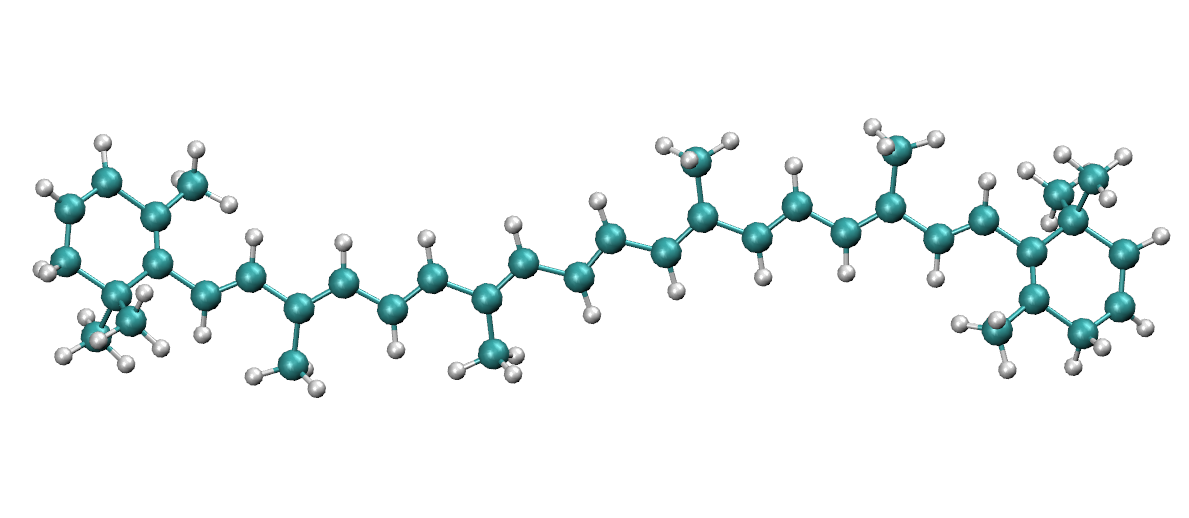
\includegraphics[width=\plotwidth]{images/caroteno.png}
   \caption{Render de caroteno}
   \label{fig:render-caroteno}
\end{figure}


